\documentclass[UTF8]{ctexart}
\usepackage{bookmark}
\usepackage{geometry}
\usepackage{hyperref}
\geometry{a4paper,scale=0.8}
\usepackage{ctex}
\usepackage{booktabs}
\usepackage{array}
\usepackage{fancyhdr}
\pagestyle{fancy}
\fancyhf{}
\renewcommand\footrulewidth{1pt}
\lhead{\textit{王铠泽}}
\rhead{\textit{PB18020766}}
\chead{\href{mailto:volar@mail.ustc.edu.cn}{\textit{volar@mail.ustc.edu.cn}}}
\rfoot{\href{http://en.ustc.edu.cn/}{\textit{中国科学技术大学}}}
\lfoot{\textit{\today}}
\usepackage{graphicx}
\usepackage{float}
\usepackage{subfigure}
\fancyfoot[C]{\textit{\thepage}}


\begin{document}

	\centering\textbf{\LARGE{计算物理A第十四次作业}}
	
	\pagenumbering{arabic}
	\textit{王铠泽\qquad PB18020766}
	
		
	\section{作业题目}
	
	\begin{itemize}
	\item	一篇应用MCMC方法研究聚乙烯小球自组装结构的研究论文“Formation of wafer-
	scale monolayer close packed polystyrene spheres template by thermally assisted self-assembly”在投稿某刊物后被审稿人拒稿,现作者欲以向刊物编辑申诉。请根据文章内容和审稿人评审意见,撰写申诉理由(你认为,作者在文中阐述的方法和
	概念以及审稿人的评论意见有哪些是合理的,哪些是需要修正的,或者哪些是需
	要进一步阐明的)。进一步,如果你是作者的话,你将如何进行该工作以及建立
	模型?
	\end{itemize}

	\section{文章摘要}
	
	\begin{flushleft}
		本文提出通过旋涂和热处理结合的方式实现高质量的密堆自组装聚苯乙烯小球阵列在晶片尺寸规模 (wafer-scale)上的量产。作者声称经由蒙特卡洛抽样方法对传统自组装理论进行了补充,得到了实验中热处理的最佳温度,为制备过程提供了很大的便利。
	\end{flushleft}
	
	\section{评论和意见}
	
	\begin{enumerate}
		\item \textbf{理论模型中相互作用只考虑入和最近邻核(nucleus)的作用不合理}
		
		在接近最终的构型过程中,球与球之间是存在着紧密排布的情形,这时最近邻核可能不止一个。再者,此时的液面形变导致的作用力(capillary force)由于曲率减小可能不是简单地随距离速降的一个函数,所以只做最近邻截断可能会出现问题。
		
		再者,本文的模型本身是想讲多体问题(每个球和球之间相互作用都计入)完全由几个分布较为稀疏的随机选取的核来代替。这一点的合理性有待质疑,在物理上的对应不是十分清晰。我的想法和评审一样是no guarantee。
		
		如果我是作者,可能会更加细致地对不同构型阶段采取更为精细的,并且更有物理意味(例如引入一个平均吸引场)来处理这个问题。
		
			\item \textbf{相互作用具体形式的参数问题}
		
		评审也提到关于相互作用的形式假设本身就存在问题。而我觉得存在更大问题的是这些参数视为温度函数是如何确定的问题。文中的相互作用中的$Q$由下式确定:
		
		
		\begin{figure}[H]
			\centering  %图片全局居中
			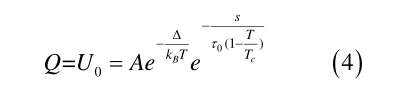
\includegraphics[width=2in]{2}
		\end{figure}	
		
		很显然,势垒$\Delta$和弛豫时间$\tau_0$应该是温度的函数,但是具体是什么函数,作者也没有指出。如果直接当成常数计算那是更加不合理。	
		
		另一个很让人费解的是出现在指数上的$Metropolis$抽样的步数$s$。我们知道,$Metropolis$抽样是对平衡构型的抽样,它的步数代表的并不是时间先后,仅仅是抽样的一个个中间过程,物理上是没有意义的。所以将其置于指数上作为随时间衰减的意思来用是错误的,这可能也是评审让作者回去多看看书的原因。而作者最后在申诉信中回复的时候似乎避重就轻,没有意识到上述问题。
		
		\item \textbf{系统能量变化令人费解}
		
		在补充材料中,可以找到系统能量随着步数变化如下:
		
		\begin{figure}[H]
			\centering  %图片全局居中
			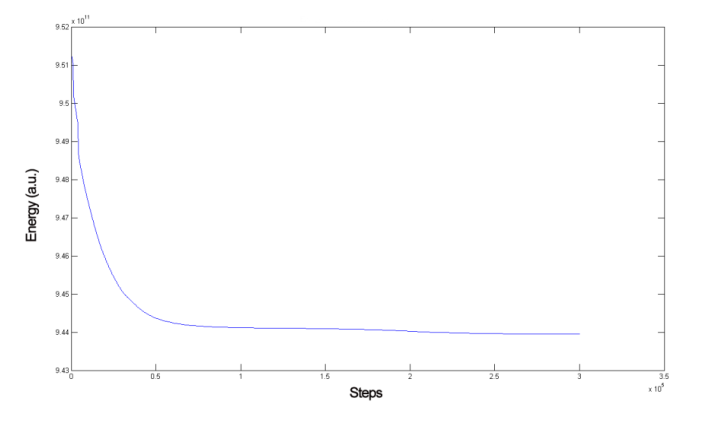
\includegraphics[width=4in]{3}
		\end{figure}
		
		按作者自设,势能$Q$应该是指数下降的,能量最终达到随着步数不变的稳态实在是令人费解。我觉得要么是算法笔误,要么是计算结果完全错误。
		
		如果我是作者,应该好好检查一边算法和程序再发表。
		
		\item \textbf{三角网格模型本身带来信息的缺失}
		
		在引入相互作用之后,作者讲小球的构型格点化,变为离散的三角网格。虽然结果上可以模拟得到密排的小球图像,但是存在对实际实验严重的信息丢失。
		
		首先,网格模型中是体现不出球堆叠的情况,没有设置重复占据(over occupied)的情形。这对后续抽样时后的步进选择造成比较大的影响。要是我是作者,我会设置好网格上的格点被多重占据对应能量,参与到抽样过程中去,而不是每次只占据空格点。
		
		再次,网格模型完全体现不出实验中自组装阵列畴与畴之间错位的情形。就算是作者得到的所谓缺陷,空隙始终也只是遵循着三角格子一定排布的空隙。详见下图这种情形:
		
		
		\begin{figure}[H]
			\centering  %图片全局居中
			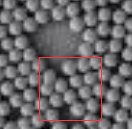
\includegraphics[width=2in]{1}
		\end{figure}		
		
		上图中红框中这种错位是摸拟所无法得到的。
		
		如果我来处理这个问题,比较好的解决方法是牺牲简单性,直接放弃网格方法,采用二维平面上自由运动的方式来模拟。
		
	
	\item \textbf{方法论可能存在根本问题}
	
	$Metropolis$抽样是对平衡构型的抽样。直接当作正则系综处理就是默认分布是$Boltzmann$分布,但是自组装是发生于远离平衡态的动力学过程,甚至是$Boltzmann$输运方程都无法准确描述的。如此抽样方法本身是否合理实在有待商榷。
	
	如果我是作者,可能我会采用MD(分子动力学模拟)这种 bottom-up 的方法来更摸拟远离平衡态的演化。
	
	\item \textbf{SEM 图像傅里叶变换处理存在局限}
	
	对SEM图像做图像处理(FT变换)得到几个谐波分量,测量随温度变化图像来表征球与球之间密堆质量在数学上是正确的,但是实际中是很容易受实验条件影响的方式。本身实际的结构一定是$x-y$平面上各向异性的,所以拍摄角度不确定、图片像素排列方向不一样就会带来谐波计算的影响,在想要比较精确地确定有序度时可能存在问题。
	
	我建议是采用其他方式来衡量密堆度,例如计算对于一个固定球,某一固定理论晶面上实际球和理论球的比较。
	
	\item \textbf{一些文章处理上的问题}
	
	多次提到$45C^\circ$是最佳的温度,但是缺鲜有展示此时的构形,SEM图像等。
	
	若我是作者,如果我坚信自己的计算没有问题,应该多放出在这个最佳温度附近的结果。
	
	\item \textbf{其他}
	
	经查,这篇文章在删去全部的计算内容 ,改进了实验方法后发表在 $ Langmuir $ 杂志上 ($ Langmuir $ 2013, 29, 14017---14023)。侧面说明了这部分的工作是存在问题的。
		
	\end{enumerate}
	
	
	
	
	

	

\end{document}